\documentclass[runningheads]{llncs}
\usepackage[T1]{fontenc}
\usepackage{graphicx}
\usepackage{amsmath,amssymb}
\usepackage{booktabs}
\emergencystretch=2em
\setlength{\textfloatsep}{8pt plus 2pt minus 2pt}
\setlength{\floatsep}{6pt plus 2pt minus 2pt}
\setlength{\intextsep}{6pt plus 2pt minus 2pt}
\setlength{\abovecaptionskip}{3pt}
\setlength{\belowcaptionskip}{0pt}
\usepackage[hidelinks]{hyperref}

\begin{document}

\title{Trust the Edge, Doubt the Arrow: Auditing Validation Signals for Text-Mined Clinical Causal Knowledge Graphs}
\titlerunning{Trust the Edge, Doubt the Arrow}

% Author information is intentionally omitted for double-anonymous review.
\author{}
\authorrunning{}
\institute{}

\maketitle

\begin{abstract}
Clinical notes contain many causal statements, and recent causal retrieval-augmented generation (RAG) systems use text-mined causal knowledge graphs (KGs) to ground clinical reasoning. However, such graphs should be treated as causal candidate graphs rather than confirmed causal graphs. Each extracted causal assertion must be audited for patient-level EHR support and directional reliability. We construct a directed graph of causal candidates from 328{,}839 MIMIC-IV discharge summaries using LLM extraction and UMLS normalization. We then audit three validation signals against SemMedDB as an independent reference: within-admission co-occurrence \emph{lift}, cross-admission diagnosis-coding \emph{temporal precedence}, and \emph{literature corroboration}. The audit reveals a consistent asymmetry. Co-occurrence lift filters unsupported co-mention candidates and provides useful EHR support evidence, but it does not establish causal truth. Diagnosis-coding order is a weak direction signal: on the 686 candidates where it commits, it reaches only 54.2\% agreement with SemMedDB, below the extractor's 69.4\% on the same subset. Literature corroboration provides independent direction evidence but covers only 30.4\% of candidate relations. A cross-release replication on MIMIC-III recovers the same pattern: extractor direction remains stable (70.5\% vs.\ SemMedDB), whereas coding-order temporal direction remains near chance (50.9\%). These results suggest that text-mined clinical causal candidate KGs should be treated as \emph{EHR-supported but direction-uncertain}. In a leakage-controlled causal QA benchmark, lift-only causal retrieval reaches 35.7\% overall accuracy, while a conservative causal-demotion policy reaches 37.2\% and reduces unsupported hallucinated answers from 17.3\% to 6.1\% at fixed retrieval recall. We provide an anonymous artifact with code, aggregate summaries, and scripts to regenerate restricted outputs.

%Clinical notes contain many causal statements, and recent causal retrieval-augmented generation (RAG) systems use text-mined causal knowledge graphs (KGs) to ground clinical reasoning. Such graphs should not be read as confirmed causal graphs. An extracted causal assertion must be audited for patient-level EHR support and for direction. We construct a directed graph of causal candidates from 328{,}839 MIMIC-IV discharge summaries using LLM extraction and UMLS normalization. We then audit three support signals against SemMedDB as an independent reference: within-admission co-occurrence \emph{lift}, cross-admission diagnosis-coding \emph{temporal precedence}, and \emph{literature corroboration}. The audit shows a consistent asymmetry. Co-occurrence lift filters unsupported co-mention candidates and is useful as EHR support evidence, but it does not prove causal truth or confirm that a causal relation exists. By contrast, diagnosis-coding order is a weak direction signal: on the 686 candidates where it commits, it reaches only 54.2\% agreement with SemMedDB, below the extractor's own 69.4\% on the same subset. Literature corroboration provides independent direction evidence but covers only 30.4\% of all candidate relations. A cross-release replication on MIMIC-III recovers the same pattern: extractor direction remains stable (70.5\% vs.\ SemMedDB), whereas coding-order temporal direction remains near chance (50.9\%). These results suggest that text-mined clinical causal candidate KGs should be treated as \emph{EHR-supported but direction-uncertain}, not as confirmed causal graphs. In a leakage-controlled causal QA benchmark, lift-only causal retrieval reaches 35.7\% overall accuracy, and a conservative causal-demotion policy reaches 37.2\% while reducing unsupported hallucinated answers from 17.3\% to 6.1\% at fixed retrieval recall. We provide an anonymous artifact with code, aggregate summaries, and scripts to regenerate restricted outputs.

\keywords{Clinical causal knowledge graph \and Knowledge graph auditing \and Retrieval-augmented generation \and Electronic health records \and Clinical NLP.}
\end{abstract}

\section{Introduction}
Mining causal relations from clinical narratives (``hepatic encephalopathy \emph{due to} alcoholic cirrhosis'') can produce causal candidate KGs for clinical reasoning. Recent \emph{causal RAG} retrieves over text-mined causal graphs so that evidence carries direction~\cite{wang2025causalrag}. These systems must decide which extracted candidates are reliable enough to retrieve. That decision has two parts: whether an LLM-extracted causal assertion has patient-level EHR support, and whether its direction has independent support. An LLM reading notes can emit clinically plausible causal assertions, unsupported co-mentions (``chest pain $\rightarrow$ abdominal pain''), and reversed candidates. A natural audit strategy is to use structured EHR signals: keep candidate relations whose endpoints co-occur more than expected and orient them by the order in which diagnoses appear over time. Yet these assumptions are rarely tested against an external reference. Unsupported candidates add retrieval noise, while misdirected candidates can lead a system to answer a causal question with a downstream consequence rather than an upstream cause. We therefore ask which signals can support an extracted relation and which can provide usable direction evidence.%An unsupported candidate adds retrieval noise, and a misdirected candidate can make a system answer ``what caused this patient's bleeding?'' with a downstream consequence. We therefore ask which of three signals, co-occurrence lift, cross-admission temporal order, and literature corroboration, can provide EHR support for an extracted relation and which can supply usable direction evidence.

%We build a directed causal candidate KG from 328K MIMIC-IV discharge summaries and audit three candidate support signals against SemMedDB, 
We build a directed causal candidate KG from 328K MIMIC-IV discharge summaries and audit three validation signals against SemMedDB, a literature-derived causal-predicate database independent of our pipeline (Fig.~\ref{fig:overview}):
\begin{itemize}
\item \textbf{Co-occurrence lift} provides EHR support: it filters unsupported co-mention candidates and improves downstream causal-QA correctness.
\item \textbf{Cross-admission temporal precedence} is unreliable as an \emph{independent EHR direction signal}: against literature direction, it is correct on only 54.2\% of the candidates where it commits, worse than the extractor on the same subset (69.4\%). ICD coding order reflects \emph{discovery}, not \emph{onset}, a hazard known to structured causal discovery~\cite{shen2021causaldiscovery} that we quantify here for text-mined candidates.
%against literature direction it is right only 54.2\% of the time where it commits, worse than the extractor on the same subset (69.4\%). ICD coding order reflects \emph{discovery}, 
%\item \textbf{Literature corroboration} gives \emph{direction but only partially}: 
\item \textbf{Literature corroboration} provides \emph{direction evidence but limited coverage}: it covers 30.4\% of all candidate relations and agrees with the extractor's direction on roughly three quarters of the covered subset.
\end{itemize}

Together, these results reveal a practical asymmetry: patient-level EHR support can be screened using a simple co-occurrence signal, whereas causal truth is not established and \emph{direction} remains uncertain. We therefore treat text-mined clinical causal candidate KGs as \emph{EHR-supported but direction-uncertain}: co-occurrence lift is used to filter unsupported candidates, the extractor's direction is retained as an imperfect text-derived estimate, and coding-order time is not used to orient candidates. Rather than proposing a new generator architecture, this work provides an audit and reusable benchmark for assessing when causal candidates mined from clinical text are reliable enough to support retrieval.

Our contributions are summarized as follows.
%\smallskip\noindent\textbf{Contributions.}
\begin{enumerate}
\item \textbf{A patient-grounded causal QA benchmark} with leakage-controlled, dual-signal reference answers. The benchmark pairs clinician-stated causal assertions with EHR support, making it a targeted test bed for support-filtered causal retrieval rather than a claim of causal ground truth.
\item \textbf{A systematic audit} of three validation signals against independent literature evidence, yielding the \emph{EHR-supported, direction-uncertain} asymmetry. Co-occurrence lift filters unsupported candidates, while cross-admission coding order is near chance and literature corroboration is coverage-limited.
% \item \textbf{A reproducible causal candidate KG construction pipeline} for 328K patient discharge notes (LLM~+~UMLS), with per-candidate audit metadata (lift, temporal, SemMedDB) and a cross-release MIMIC-III replication of the audit.
\item \textbf{A reproducible pipeline for clinical causal candidate KG construction} from 328K discharge notes, combining LLM extraction, UMLS normalization, per-candidate audit metadata, and cross-release replication on MIMIC-III.
%\item A controlled causal-RAG study in which lift-only retrieval is the honest base after the temporal-direction audit. 
\item \textbf{A controlled causal-RAG study} in which lift-only retrieval serves as the audit-consistent baseline after the temporal-direction audit. A conservative causal-demotion policy preserves recall, substantially reduces unsupported hallucinated answers, and gives a small non-significant accuracy trend.
\end{enumerate}
%Together these results expose an asymmetry: patient-level EHR support can be screened with a simple signal, but causal truth is not proven and \emph{direction} remains uncertain. We therefore treat text-mined clinical causal candidate KGs as \emph{EHR-supported but direction-uncertain}: use co-occurrence lift to filter unsupported candidates, retain the extractor's direction as a calibrated but imperfect estimate, and avoid orienting candidates by coding-order time. The contribution is not a new generator architecture. It is an audit and reusable benchmark that asks when a causal candidate graph mined from clinical text is useful enough for retrieval.

%The main value of the study is diagnostic: it identifies which support signal can be used before extracted causal candidates are retrieved, rather than treating the QA delta as the sole contribution.

\begin{figure}[!htbp]\centering
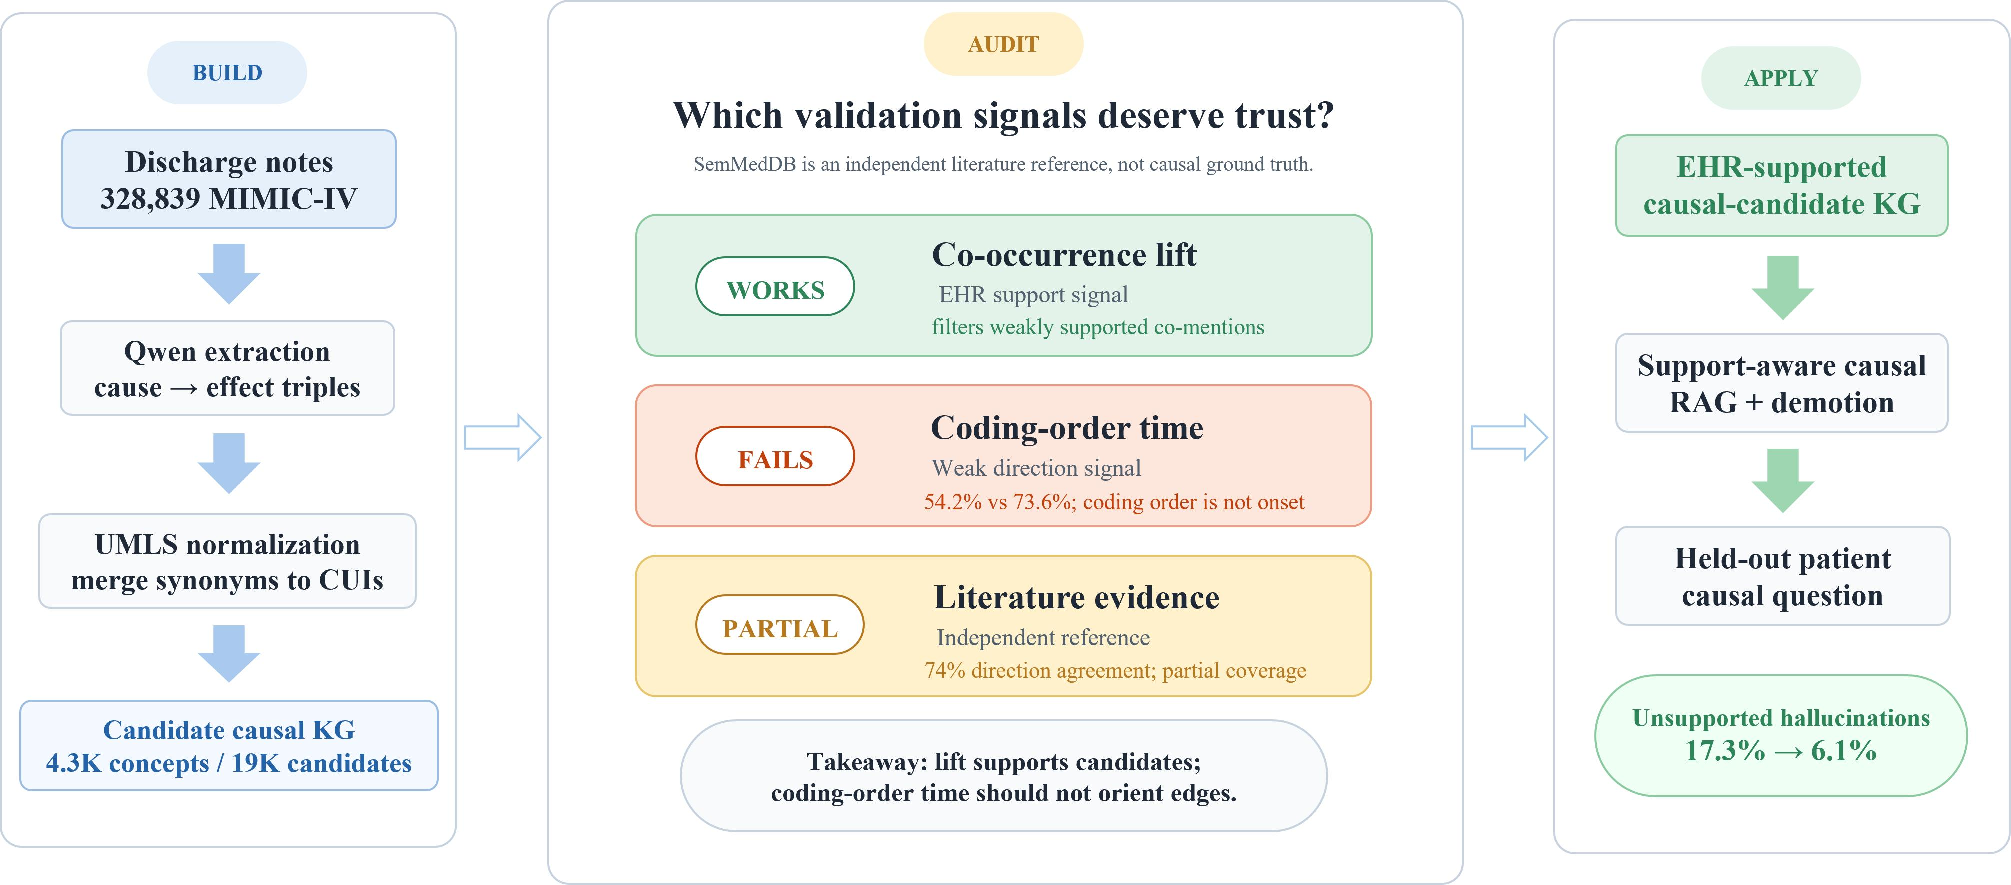
\includegraphics[width=\textwidth]{fig1.pdf}
%\caption{Overview. \textbf{Build:} a graph of causal candidates is mined from clinical notes (Qwen + UMLS). \textbf{Audit:} each candidate relation is scored against independent literature evidence (SemMedDB): co-occurrence lift filters unsupported candidates, cross-admission coding-order temporal precedence is unreliable as a direction signal (54.2\% vs.\ 69.4\% on the committed subset), and literature corroboration is partial. \textbf{Apply:} support-aware causal RAG uses the EHR-supported candidate graph and demotes candidates that fail the causal screen. The downstream effect emphasized here is fewer unsupported hallucinated answers at fixed recall, not a statistically significant accuracy gain over lift-only.}
\caption{Overview of the proposed audit-and-retrieval framework. \textbf{Build:} causal candidates are mined from clinical notes and normalized to UMLS concepts. \textbf{Audit:} co-occurrence lift provides EHR support, coding-order time is unreliable for direction, and SemMedDB provides partial literature corroboration. \textbf{Apply:} support-aware causal RAG retrieves from the EHR-supported candidate graph and demotes candidates that fail the causal screen, reducing unsupported hallucinations at fixed recall.}
\label{fig:overview}
\end{figure}

\section{Related Work}
\noindent\textbf{Clinical KGs from text and EHR.} Clinical KG methods commonly use ontologies, co-occurrence, or patient-specific associative graphs. GRAM~\cite{choi2017gram} and KAME~\cite{ma2018kame} use ICD ontologies; Rotmensch et al.~\cite{rotmensch2017learning} learn disease--symptom co-occurrence graphs; LLMs extract KGs from notes~\cite{nadkarni2023llmkg}; and GraphCare~\cite{jiang2024graphcare} builds personalized KGs for prediction. These graphs are mainly ontological or associative, not audited causal candidates.
%GRAM~\cite{choi2017gram} and KAME~\cite{ma2018kame} inject ICD ontologies. Rotmensch et al.~\cite{rotmensch2017learning} learn disease-symptom graphs by co-occurrence; LLMs extract KGs from notes~\cite{nadkarni2023llmkg}; and GraphCare~\cite{jiang2024graphcare} builds per-patient KGs. These edges are usually ontological or associative, with no causal direction and no audit against patient outcomes.

\noindent\textbf{Causal KGs in medicine.} Biomedical causal KGs often use literature-scale predications such as SemMedDB~\cite{kilicoglu2012semmeddb}, combine literature relations with EHR evidence~\cite{nordon2019building}, or evaluate literature-derived graphs in EHR case studies~\cite{lyu2023dnkg}. Other work studies adverse drug effects~\cite{ade2026causalkg}, structured EHR causal discovery~\cite{shen2021causaldiscovery}, and causal GNNs~\cite{causalgnn2025survey}. A key challenge is validation: diagnosis timestamps often reflect documentation rather than onset, so naive temporal order can misorient relations~\cite{shen2021causaldiscovery,doutreligne2024causal}. We instead audit support and direction signals for causal candidates mined from patient narratives.%Biomedical causal KGs often draw on literature-scale semantic predications, such as SemMedDB~\cite{kilicoglu2012semmeddb}, combine literature graphs with EMR evidence~\cite{nordon2019building}, or evaluate literature-derived causal KGs in EHR case studies~\cite{lyu2023dnkg}. Others use biomedical KGs to analyze adverse drug effects~\cite{ade2026causalkg}, discover causal structure from structured variables~\cite{shen2021causaldiscovery}, or survey causal GNNs~\cite{causalgnn2025survey}, noting a ``validation crisis''~\cite{ade2026causalkg,doutreligne2024causal}. A recurring hazard is that EHR diagnosis timestamps reflect \emph{documentation} rather than \emph{onset}, so naive temporal order can mis-orient candidate relations. Onset-correction methods are proposed to mitigate it~\cite{shen2021causaldiscovery}. LLMs are now used to extract causal relations from medical text~\cite{causalextract2024llm,nadkarni2023llmkg}, and SemMedDB is an established reference for evaluating biomedical causal relations~\cite{kilicoglu2012semmeddb}. None of these mine causal candidates from \emph{patient narratives} and audit which signals provide EHR support or recover direction.

\noindent\textbf{KG-augmented prediction.} GraphCare~\cite{jiang2024graphcare}, KARE~\cite{kare2025}, RAM-EHR~\cite{xu2024ramehr}, MedText~\cite{lu2021medtext}, MM-STGNN~\cite{tang2023multimodal}, and KAT-GNN~\cite{katgnn2025} use graph structure to improve EHR outcome prediction. They optimize prediction rather than auditing whether extracted relations have EHR support or reliable direction.
%couple ontology or co-occurrence graphs with EHR for outcome prediction. They do not audit support or direction signals.

\noindent\textbf{RAG, GraphRAG, causal RAG.} GraphRAG~\cite{edge2024graphrag}, Medical Graph RAG~\cite{medgraphrag2024}, and ontology-grounded clinical QA~\cite{llmkg2024biomed} retrieve KG evidence to reduce hallucination. CausalRAG~\cite{wang2025causalrag} retrieves over a text-extracted causal graph, so retrieved evidence carries direction. However, these systems usually assume the retrieved graph is reliable. We study the preceding question: before causal candidates are retrieved, which ones have patient-level support, and which directions have independent support? A raw causal-RAG variant is therefore used as a reference point in our evaluation. %GraphRAG~\cite{edge2024graphrag}, Medical Graph RAG~\cite{medgraphrag2024}, and ontology-grounded clinical QA~\cite{llmkg2024biomed} curb hallucination by retrieving over a KG. CausalRAG~\cite{wang2025causalrag} retrieves over a \emph{causal} graph extracted from text, so the evidence carries direction. In these settings the retrieved graph is usually assumed to be correct, either because an ontology is curated or because LLM and literature relations are accepted as extracted. A noisy or misdirected candidate can then propagate into the answer. We study the preceding question: which extracted candidates have patient-level support, and which directions have independent support? We use a raw causal-RAG variant as our reference point.

\noindent\textbf{Clinical QA benchmarks.} Existing EHR QA benchmarks, such as EHRNoteQA \cite{kweon2024ehrnoteqa}, EHRXQA~\cite{ehrxqa2023}, EHRSQL~\cite{lee2022ehrsql}, and emrQA~\cite{pampari2018emrqa}, mainly evaluate factual QA over notes, tables, or structured records. General-domain causal QA exist~\cite{yang2022causalreasoning}, but are not clinical or patient-grounded. We address this gap with a benchmark that pairs patient-grounded causal questions with reference answers supported by both clinician-stated causal assertions and structured EHR evidence.%EHRNoteQA~\cite{kweon2024ehrnoteqa}, EHRXQA~\cite{ehrxqa2023}, EHRSQL~\cite{lee2022ehrsql}, emrQA~\cite{pampari2018emrqa} target factual/table questions; general-domain causal reasoning QA exists~\cite{yang2022causalreasoning} but is not clinical or patient-grounded. None pair \emph{causal} questions with reference answers that require both textual assertion and EHR support. We contribute one.

\noindent\textbf{Positioning.} Table~\ref{tab:position} positions our work against representative systems along five axes. Existing clinical GraphRAG systems mainly use associative or ontology-based edges; CausalRAG studies directed retrieval outside patient EHR narratives; and literature-derived causal KGs provide causal predicates but are not mined from patient notes or audited for candidate direction. In contrast, our study jointly mines directed causal candidates from patient narratives, filters them with structured-EHR support, audits direction signals, and evaluates them with a patient-grounded causal QA benchmark.%summarizes how our work differs from representative prior systems along five axes. The present study combines four elements that are usually treated separately: directed causal candidate mining from patient narratives, structured-EHR support filtering, direction-signal auditing, and a causal QA benchmark.

\begin{table}[!htbp]
\centering
%\caption{Positioning vs.\ representative prior work along five axes ($\checkmark$~yes, $\sim$~partial, $\times$~no). GraphCare / Medical Graph RAG use associative or ontology edges; CausalRAG is general-domain; literature-derived causal KGs are not mined from patient narratives and do not audit candidate direction, even when they use EMR filtering or EHR case-study evaluation. Ours mines directed causal candidates from patient notes, filters them with co-occurrence lift, audits direction against SemMedDB, and defines a causal QA benchmark.}
\caption{Positioning against representative prior work. \checkmark{} indicates yes, $\sim$ partial, and $\times$ no. Ours is the only setting that combines directed causal candidate mining from patient narratives, structured-EHR support filtering, direction-signal auditing, and a patient-grounded causal QA benchmark.}
\vspace{-0.2cm}
\label{tab:position}
\setlength{\tabcolsep}{2pt}\footnotesize
\resizebox{\textwidth}{!}
{%
\begin{tabular}{lccccc}\toprule
 & Directed & Patient & EHR & Direction & QA \\
 & Candidates & Text & Support & Audited & Benchmark \\\midrule
GraphCare~\cite{jiang2024graphcare}, Med.\ GraphRAG~\cite{medgraphrag2024} & $\times$ & $\sim$ & $\times$ & $\times$ & $\times$ \\
CausalRAG~\cite{wang2025causalrag} & $\checkmark$ & $\times$ & $\times$ & $\times$ & $\times$ \\
Lit.\ causal KGs~\cite{kilicoglu2012semmeddb,nordon2019building,lyu2023dnkg,ade2026causalkg} & $\checkmark$ & $\times$ & $\sim$ & $\times$ & $\times$ \\
\textbf{Ours} & $\checkmark$ & $\checkmark$ & $\checkmark$ & $\checkmark$ & $\checkmark$ \\\bottomrule
\end{tabular}}
\vspace{-0.3cm}
\end{table}

\section{Building the Candidate Causal KG}
\noindent\textbf{Extraction.} %A discharge summary mixes a free-text narrative with templated patient-instruction boilerplate (``call your doctor if\ldots''); the latter repeats across notes and otherwise dominates raw edge frequency. We therefore restrict extraction to the History of Present Illness and Hospital Course sections (including ``Brief Hospital Course'')
A discharge summary mixes free-text clinical narrative with templated patient-instruction boilerplate (``call your doctor if\ldots''), which repeats across notes and can dominate raw edge frequency. We therefore restrict extraction to the History of Present Illness and Hospital Course sections, including ``Brief Hospital Course'', and prompt Qwen2.5-7B-Instruct~\cite{qwen2025} (AWQ, vLLM~\cite{kwon2023vllm}, temperature~0) to emit a JSON array of \texttt{\{"cause","effect"\}} pairs for each note. Over the 328{,}839 MIMIC-IV-Note discharge summaries~\cite{johnson2023mimicnote}, 79.5\% yield $\geq$1 triple, giving 1.31M triples (3.98 per note) and 1.17M unique surface edges. The unique-edge distribution is heavy-tailed: 96.4\% occur exactly once. Because the singleton tail is dominated by hyper-specific or noisy spans, the candidate KG retains only edges attested in $\geq$2 notes (42{,}798). Singleton extractions are excluded from the KG but retained as per-note provenance for benchmark grounding.%Because the singleton tail is dominated by hyper-specific or noisy spans, we keep only edges attested in $\geq$2 notes (42{,}798), retaining the singletons as per-note provenance for benchmark grounding.

\noindent\textbf{Normalization.} %Surface phrases are noisy (synonyms, abbreviations, modifiers), so we link each cause span and effect span to a UMLS~\cite{bodenreider2004umls} Concept Unique Identifier 
Surface phrases contain synonyms, abbreviations, and modifiers, so we link each cause and effect span to a UMLS Concept Unique Identifier (CUI)~\cite{bodenreider2004umls} with a scispaCy~\cite{neumann2019scispacy} candidate generator. We accept the top candidate when cosine similarity is $\geq0.80$ and its semantic types are not in a non-clinical blocklist, thereby collapsing co-referring surface forms into concept nodes. Compared with a rule-based cue-phrase extractor, LLM extraction more than doubles the UMLS link rate (49.3\% vs.\ 21.9\%) and increases the giant connected component from 86.9\% to 97.1\% at comparable graph size (Table~\ref{tab:kg}), suggesting that LLM-extracted spans are more concept-like. Table~\ref{tab:kg} reports statistics on the full pre-split corpus. After the patient-level split used for leakage control (\S\ref{sec:qa}), the train-only KG used for retrieval and release contains 3{,}899 concept nodes and 16{,}273 directed edges.
%co-referring surface forms thereby collapse to one concept node. Linking raises the giant connected component from 86.9\% to 97.1\% and more than doubles the link rate versus a rule-based cue-phrase extractor (49.3\% vs.\ 21.9\%) at comparable graph size (Table~\ref{tab:kg}), confirming that LLM spans are cleaner concepts. Table~\ref{tab:kg} reports the full pre-split graph. After a patient-level split for leakage control (\S\ref{sec:qa}), the train-only KG used for retrieval and release has 3{,}899 concept nodes and 16{,}273 directed edges.

\begin{table}[!htbp]\centering
\caption{Candidate-KG construction on the full pre-split corpus: rule-based vs.\ LLM extraction.}
%\caption{Rule-based vs.\ LLM extraction for candidate KG construction.}
\label{tab:kg}\footnotesize
\setlength{\tabcolsep}{4pt}
\begin{tabular}{lrr}\toprule
Metric & Rule-based & LLM(ours) \\\midrule
Raw surface edges & 142{,}890 & 1{,}173{,}644 \\
UMLS link rate & 21.9\% & \textbf{49.3\%} \\
CUI nodes & 8{,}572 & \textbf{4{,}318} \\
CUI edges & 19{,}171 & 19{,}035 \\
Giant component & 92.3\% & \textbf{97.1\%} \\
Lift-supported candidates & 736 & \textbf{2{,}047} \\\bottomrule
\end{tabular}\end{table}

\section{The Support and Direction Audit}\label{sec:audit}
We score three validation signals against two questions: whether an extracted causal candidate has patient-level EHR support, and whether its \emph{direction} has independent support. As an independent reference, we use SemMedDB v43~\cite{kilicoglu2012semmeddb}, a repository of 115.5M semantic predications extracted from PubMed. We keep the causal predicates \textsc{causes}, \textsc{predisposes}, and \textsc{induces}, read the subject$\rightarrow$object orientation as the literature's causal direction, and restrict the analysis to predications whose subject and object CUIs both occur in our KG. When both orientations are attested, we use the majority direction by citation support. This yields literature causal evidence for 4{,}943 KG candidate relations. Because SemMedDB is imperfect (relaxed $F_1\approx0.5$~\cite{kilicoglu2012semmeddb}), we treat it as an independent reference rather than ground truth, and compare each signal against both SemMedDB and the extractor's text-derived direction.%conclusion with the extractor's own text-derived direction.

\smallskip\noindent\textbf{Experimental logic.} The audit and the downstream QA study answer different questions. The audit evaluates which validation signal can support candidate existence and which can recover direction. Each signal is reported by coverage and, when it commits to a direction, agreement with SemMedDB. The QA study then tests whether the useful part of the audit, support filtering by lift, improves causal RAG under a controlled benchmark. All QA systems share the same generator, prompt, and retrieval budget; differences therefore reflect the retrieved evidence rather than the surrounding model setup. %so differences isolate .
%answer which support question. 

\subsection{Co-occurrence lift provides EHR support}
We map ICD diagnoses to CUIs and, for candidate $A\rightarrow B$, compute the within-admission $\mathrm{lift}=P(B\mid A)/P(B)$. A candidate is treated as \emph{supported} when $\mathrm{lift}>1$ with sufficient co-occurrence; 2{,}047 LLM candidates meet this criterion. Lift is \emph{symmetric}, so it measures association strength rather than direction or causal truth. It demotes weakly supported co-mentions: ``chest pain $\rightarrow$ abdominal pain'' (two common symptoms with high base rates) is not supported ($\mathrm{lift}\approx1$), whereas ``alcoholic cirrhosis $\rightarrow$ hepatic encephalopathy'' is strongly supported ($\mathrm{lift}=65$). Section~\ref{sec:qa} shows that retrieving over the lift-supported subgraph improves downstream causal-QA correctness. Co-occurrence lift is therefore useful for EHR support filtering, not causal proof or orientation.

\subsection{Cross-admission temporal precedence does not recover direction}
We hypothesized that across admissions a cause is coded \emph{before} its effect. We test this on the 4,943 candidate relations with SemMedDB direction evidence, comparing the extractor's text-derived direction with the direction implied by cross-admission coding order. As temporal precedence often abstains, we report both committed-subset accuracy and a coverage-adjusted paired comparison.%We test this: for the 4{,}943 candidates with SemMedDB direction, compare the extractor's surface direction and temporal precedence against the literature reference (Table~\ref{tab:audit}).

%Table~\ref{tab:audit} and Fig.~\ref{fig:audit} summarize the result. Temporal precedence commits on only 686 candidates and reaches 54.2\% agreement with SemMedDB, compared with 69.4\% for the extractor's direction on the same subset. Over all 4,943 SemMedDB-covered candidates, treating abstentions as failures to recover direction, the extractor is correct far more often than temporal precedence (LLM-only-right: 3,365; temporal-only-right: 100; McNemar $p \ll 0.001$). The error decomposition in Fig.~\ref{fig:audit} further shows that temporal reversals are mostly harmful: among 304 reversed verdicts, only 100 are true corrections, whereas 204 are false reversals, including asthma$\rightarrow$wheezing, hemorrhage$\rightarrow$anemia, and abdominal-pain$\rightarrow$appendicitis.
Table~\ref{tab:audit} and Fig.~\ref{fig:audit} show that temporal precedence is a weak direction signal. It commits on only 686 candidates and reaches 54.2\% agreement with SemMedDB, below the extractor's 69.4\% on the same subset. Over all 4,943 candidates, treating abstentions as failures to recover direction, the extractor is correct far more often than temporal precedence (LLM-only-right: 3,365; temporal-only-right: 100; McNemar $p \ll 0.001$). Fig.~\ref{fig:audit} further shows that most temporal reversals are harmful: among 304 reversed verdicts, only 100 are true corrections and 204 are false reversals.

\begin{table}[!htbp]\centering\caption{Direction-signal accuracy vs.\ SemMedDB ($n=4{,}943$ candidate relations). Temporal precedence abstains on 86\% of candidates; on the 686 where it commits it is below the extractor's own direction and near chance.}\label{tab:audit}\footnotesize
\begin{tabular}{lc}\toprule
Direction signal & Acc.\ vs.\ SemMedDB \\\midrule
Raw LLM extraction direction & \textbf{73.6\%} \\
Temporal precedence (committed, $n{=}686$) & 54.2\% \\
LLM direction on those 686 & 69.4\% \\\bottomrule
\end{tabular}\end{table}

%McNemar (temporal vs.\ LLM): LLM-only-right 3{,}365 vs.\ temporal-only-right 100, $p\approx0$. This test scores temporal precedence as an independent directioner over all 4{,}943 candidates; abstention is counted as failing to recover the literature direction. Of temporal's 304 ``reversed'' verdicts, only 100 are true corrections while 204 are false reversals (e.g.\ asthma$\rightarrow$wheezing, hemorrhage$\rightarrow$anemia, abdominal-pain$\rightarrow$appendicitis flipped; Fig.~\ref{fig:audit}).

\begin{figure}[!htbp]\centering
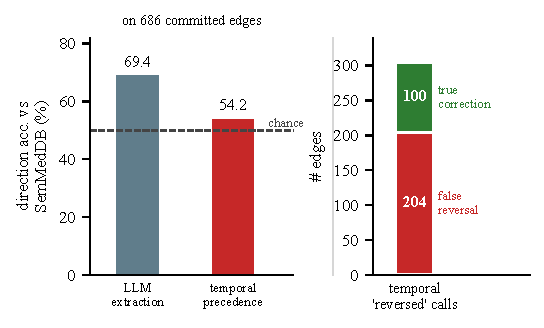
\includegraphics[width=0.78\textwidth]{fig_audit.pdf}
\caption{Direction-signal audit. \emph{Left:} on the 686 candidate relations where cross-admission temporal precedence commits to a direction, it agrees with SemMedDB less often (54.2\%) than the extractor's own direction (69.4\%) and barely above chance. \emph{Right:} of temporal's 304 ``reversed'' verdicts, 204 are false reversals (coding artifacts) and only 100 are true corrections.}
\label{fig:audit}
\end{figure}

\noindent\textbf{Interpretation.} 
%The failure mode is clinically plausible: ICD coding order reflects documentation and discovery rather than disease onset. Chronic conditions may be co-coded across encounters, while symptoms, complications, and findings are often coded when they are recognized rather than when they began. This timestamp hazard is known in structured EHR causal discovery, where onset correction is used to distinguish incident from prevalent diagnoses~\cite{shen2021causal}. Our result quantifies the same hazard for orienting text-mined causal candidates: uncorrected coding-order time is near chance and worse than the extractor's text-derived direction.
ICD coding order reflects \emph{discovery/coding}, not \emph{onset}: chronic conditions are co-coded, and findings are coded at the encounter in which they are discovered. This timestamp hazard is known to structured causal discovery, where onset-correction (distinguishing incident from prevalent diagnoses) is the proposed remedy~\cite{shen2021causaldiscovery}. Here we quantify the same hazard for orienting text-mined causal candidates, where the temporal signal is barely above chance and below the extractor's own direction. SemMedDB itself has direction noise, but it and the extractor are both text-derived and agree on 73.6\% of all SemMedDB-covered directions, while the structured temporal signal correlates with neither. Applying onset-correction to the temporal signal is left to future work.

\noindent\textbf{Robustness.} 
%SemMedDB is not a gold standard and contains direction noise. However, the observed gap is unlikely to be explained solely by SemMedDB artifacts. The extractor and SemMedDB are independent text-mining sources and agree on 73.6\% of SemMedDB-covered directions, whereas the structured temporal signal agrees poorly and abstains on most candidates. We therefore interpret coding-order temporal precedence as an unreliable direction signal in its uncorrected form, while leaving onset-corrected temporal modeling to future work.
The McNemar comparison is paired over all 4{,}943 SemMedDB-covered candidates. Each candidate has an extractor verdict, and the temporal signal is counted as correct only if it commits to the literature direction. Abstentions are therefore failures for an independent directioner. The committed-only accuracy in Table~\ref{tab:audit} is a diagnostic subset, not the McNemar denominator. The gap is unlikely to be a SemMedDB artifact. The extractor and SemMedDB are produced by independent text-mining pipelines yet agree on 73.6\% of all SemMedDB-covered directions, whereas the structured temporal signal agrees with neither. This is the pattern expected if diagnosis-coding order carries little causal-direction information.

\subsection{Literature corroboration is useful but partial}
Among the 2{,}047 lift-supported candidates, 886 (43\% of the lift-supported subset) are also attested by SemMedDB. The attested subset agrees with the extractor's direction in 74\% of cases and covers 61\% of benchmark reference relations. Its value depends on how it is used. As a strict filter requiring both EHR-lift support and literature attestation, it would discard the remaining 1{,}161 lift-supported EHR candidates (57\%) that fall outside SemMedDB's PubMed-derived coverage. This would hurt recall. As a confidence tier, it separates high-confidence candidates (lift \emph{and} literature) from EHR-only candidates and supplies an independent direction for the subset it covers. We therefore use it as coverage-limited corroboration rather than as a strict filter.

\smallskip\noindent\textbf{Takeaway.} Co-occurrence lift provides patient-level EHR support for extracted candidates; \emph{direction} remains uncertain because coding-order time is near chance and literature covers a minority of candidates. Text-mined clinical causal candidates are therefore best treated as EHR-supported but direction-uncertain. We filter by lift, keep the extractor's direction as an uncertain estimate, and avoid orienting candidates by coding-order time.

\subsection{Putting it together: a support-filtering recipe}
The audit yields a reproducible recipe for converting raw LLM-extracted causal candidates into an EHR-supported candidate graph, without manual curation (Fig.~\ref{fig:funnel}). Starting from 42{,}798 recurrent surface candidate relations, we first normalize endpoints to UMLS concepts (\S\ref{sec:audit} reduces 16{,}151 surface nodes to 4{,}318 concepts). We then keep candidates with within-admission lift~$>1$, yielding 2{,}047 supported candidate relations, and orient each candidate by the extractor's direction rather than by coding-order time. Finally, we flag the 886 literature-corroborated candidates as a higher-confidence core and treat the remainder as EHR-only. The resulting graph has patient-level support annotations grounded in text and structured co-occurrence, without establishing causal truth. Its \emph{direction} claims retain source-aware uncertainty. Section~\ref{sec:qa} shows that this graph supports downstream causal QA retrieval, and the recipe transfers to note corpora paired with linked structured records.

\begin{figure}[!htbp]\centering
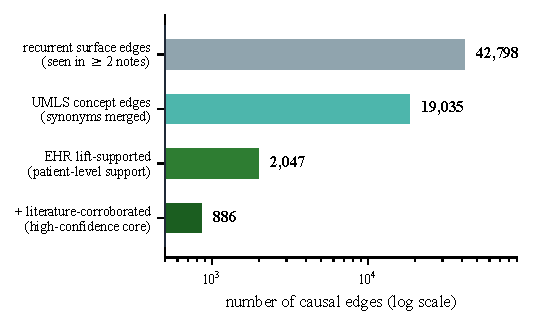
\includegraphics[width=0.72\textwidth]{fig_funnel.pdf}
\caption{The support-filtering recipe as a funnel. Recurrent LLM candidates are normalized to UMLS concepts, filtered to the EHR lift-supported subgraph, and partitioned by literature corroboration into a higher-confidence core; direction is taken from the extractor rather than coding-order time.}
\label{fig:funnel}
\end{figure}

\subsection{Cross-release replication on MIMIC-III}
To test whether the audit depends on the MIMIC-IV release, we reran the same extraction, UMLS normalization, structured-diagnosis lift support filtering, temporal analysis, and SemMedDB comparison on MIMIC-III. The replication uses 53{,}981 usable discharge-summary sections and yields 237{,}957 clean triples, 221{,}454 surface edges, and 35{,}232 CUI-level edges. Although this graph is larger and noisier than the MIMIC-IV train graph, the qualitative conclusions replicate (Fig.~\ref{fig:mimic3}): 942 of 2{,}318 diagnosis-testable candidates are lift-supported (40.6\%); SemMedDB covers 6{,}753 candidates (19.2\%); extractor direction remains aligned with SemMedDB (70.5\%, close to the 73.6\% overall MIMIC-IV extractor agreement); and coding-order direction remains near chance (50.9\%, close to the 54.2\% MIMIC-IV committed-subset result). Thus MIMIC-III strengthens the central audit claim under a different EHR release: the EHR support pattern transfers, while naive temporal orientation remains unreliable.

\begin{figure}[!htbp]\centering
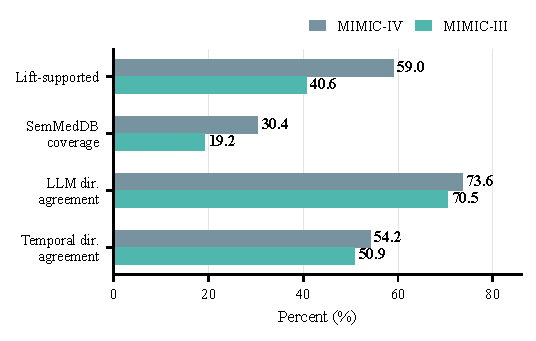
\includegraphics[width=0.78\textwidth]{fig_mimic3_replication.pdf}
\caption{Cross-release replication on MIMIC-III. Compared with the main MIMIC-IV audit, MIMIC-III has lower lift support and lower SemMedDB coverage, but the direction pattern is stable: the extractor's direction remains substantially above chance, whereas coding-order direction remains near chance.}
\label{fig:mimic3}
\end{figure}

\section{Causal QA Benchmark and Downstream Utility}\label{sec:qa}
\subsection{Benchmark}
\smallskip\noindent\textbf{Reference construction.}
A candidate relation becomes a benchmark answer only under a \emph{dual signal}. It must be stated as a cause and effect relation by the treating clinician in a \emph{held-out} note, and it must be EHR-lift-supported ($\mathrm{lift}\geq2$). This support threshold is stricter than the graph-construction threshold ($\mathrm{lift}>1$): the graph threshold keeps useful retrieval candidates, whereas the benchmark threshold reduces weak associations in the reference set. This pairing removes symptom co-mention noise that either signal alone would admit. 

\smallskip\noindent\textbf{Leakage control.}
We split the 145{,}872 patients of MIMIC-IV~\cite{johnson2023mimiciv} 85/15 by \texttt{subject\_id} (124{,}058 train / 21{,}814 test). The candidate KG is built from \emph{train} notes only, so no test patient's note contributes a candidate relation. Population-level lift may use all patients' codes, a different modality that cannot reveal an individual's text answer. Questions are drawn from \emph{test} patients and answered against the train-only candidate KG. Because lift also defines our support-filtered retrieval condition, this benchmark is a downstream utility check under the same operational support definition, not an independent proof that lift establishes causal truth.

\smallskip\noindent\textbf{Statistics and evaluation.} The benchmark pool contains 2{,}319 patient-grounded items over WHY, WHATCAUSES, and direction-discrimination templates. The downstream experiment evaluates only the forward causal-QA subset: WHY (``most likely underlying cause of \{effect\}?'') and WHATCAUSES (``what does \{cause\} most likely lead to?''), with 466 items each (932 total) over 170 EHR-supported causal candidates. We leave the direction-discrimination templates for future evaluation because the present downstream question is whether support-filtered retrieval improves answer evidence when the question direction is fixed. Each question is presented with the patient's coded problem list. To avoid a trivially solvable task, in $\sim$half of items the reference cause is not already in the coded problem list. The system must supply it from causal knowledge rather than copy it from the list. A balanced 120-item subset is human-checked for answer correctness and direction. Correctness means that the predicted concept CUI-matches the reference, or that an automatic Qwen judge confirms the same condition. Faithfulness means that the predicted concept appears in the system's retrieved evidence.

\subsection{Does EHR support filtering help causal RAG?}
\noindent\textbf{Why these baselines.} No published system exactly matches patient-grounded causal QA over an EHR-mined causal candidate graph under this support-filtering setting. Rather than compare against systems that also change the generator, chunking, or prompt, we re-implement retrieval paradigms under one harness. All systems share the same generator (Qwen2.5-7B), prompt, and retrieval budget, and differ \emph{only} in the retrieved evidence. The baselines are: (1)~\textbf{closed-book}, none; (2)~\textbf{naive TF-IDF text-RAG}, top-3 discharge-note excerpts; (3)~\textbf{SemMedDB-only}, a directed literature causal graph for external biomedical KG grounding~\cite{kilicoglu2012semmeddb}; (4)~\textbf{assoc-graph}, undirected co-occurrence neighbours in a GraphRAG-style associative retrieval setting~\cite{edge2024graphrag,medgraphrag2024,jiang2024graphcare}; (5)~\textbf{raw-causal}, the raw LLM directed candidate graph with no support filtering, as a CausalRAG-style reference~\cite{wang2025causalrag}; (6)~\textbf{lift + temporal}, the lift-supported graph after applying the audited coding-order temporal direction signal; (7)~\textbf{lift-only}, the EHR-supported candidate graph in the extractor's original direction; and (8)~\textbf{lift-only + causal demotion} (ours), which keeps the same top-12 lift candidates but moves candidates that fail the causal screen to the end of the evidence list. Thus, differences reflect the retrieval source or evidence ordering rather than changes to the generator, prompt, or retrieval budget. %Thus any difference isolates retrieved evidence ordering rather than the surrounding model.
Raw-causal directly ablates support filtering. Lift + temporal shows the cost of using the rejected coding-order direction signal: recall falls to 77.8\%. Lift-only directly ablates causal demotion.

\smallskip\noindent\textbf{Retrieval setup.}
For the graph systems, retrieval is direction-aware: a WHY question pulls the \emph{in}-edges of the asked effect (its candidate causes) and a WHATCAUSES question its \emph{out}-edges, ranked by lift, frequency, or PMID support. The top~12 are serialized into the prompt, and the lift-only systems additionally annotate each candidate with its lift. The generator returns a single condition, which we then match. Generation and judging run on a 7B open model on a private cluster, so MIMIC text does not leave the compliant environment.

\smallskip\noindent\textbf{Causal-screen demotion.} The demotion layer is a post-retrieval ordering rule, not a new retriever. Lift-only retrieval first selects the same top-12 candidates by co-occurrence lift. The causal screen is queried only for those directed pairs: for WHY, candidate cause$\rightarrow$queried effect; for WHATCAUSES, queried cause$\rightarrow$candidate effect. The screen is estimated on the training split as a new-user, incident-outcome design over structured diagnoses: the cause must occur at baseline, the effect must first appear later among outcome-naive patients, and each patient needs follow-up ($\geq$2 admissions). The adjusted risk-ratio signal uses inverse-propensity weighting for age, sex, and baseline comorbidity burden, then calibrates a $z$ score with automatically sampled negative-control diagnosis outcomes that the cause does not point to in the candidate KG; these controls are not manually chosen and do not use held-out QA answers. The implementation samples up to 20 controls per tested pair, requires at least five valid controls for calibration, and estimates a pair only when both exposure arms have at least 50 eligible patients and at least 10 incident outcome events. A candidate \emph{passes} if $z\geq1.64$, \emph{fails} if it is estimated but below that one-sided 5\% threshold, and is \emph{untested} otherwise. The cutoff, screen, and QA prompts are fixed before answer generation and are not tuned on held-out QA answers. Demotion moves failed candidates to the end of the same top-12 list while leaving pass and untested candidates in lift order; it changes ordering but cannot add or remove candidates.

\smallskip\noindent\textbf{Causal-screen coverage.}
Table~\ref{tab:screen} summarizes how often the causal screen affects the lift-only evidence lists. 
\begin{table}[!b]\centering
\caption{Causal-screen coverage and ranking effect in the lift-only top-12 retrieval lists. The screen is applied after lift-only retrieval and only reorders the selected candidates. Lower mean rank indicates earlier placement in the evidence list.}
\label{tab:screen}
\scriptsize
\setlength{\tabcolsep}{3pt}
\begin{tabular}{lrrrrr}\toprule
Screen status & Slots & \% & Unique pairs & Qs $\geq$1 & Mean rank before$\to$after \\\midrule
Pass ($z\geq1.64$) & 1{,}718 & 18.6 & 127 & 630 (67.6) & 4.63$\to$3.78 \\
Fail ($z<1.64$) & 4{,}510 & 48.7 & 494 & 807 (86.6) & 7.09$\to$8.39 \\
Untested & 3{,}025 & 32.7 & 377 & 780 (83.7) & 5.54$\to$4.08 \\
Total & 9{,}253 & 100 & -- & 932 & -- \\\bottomrule
\end{tabular}
\end{table}
Across the 932 questions, lift-only retrieval produces 9,253 top-12 candidate slots. The screen assigns 18.6\% of slots to pass, 48.7\% to fail, and leaves 32.7\% untested because of sample-size or coverage requirements. Demotion changes the evidence order in 678 questions (72.7\%) without changing the retrieved candidate set, so recall is preserved by construction. Failed candidates move down the list on average, while pass and untested candidates move upward relative to them.

\begin{table}[!htbp]\centering
%\caption{Causal QA on held-out patients (\%). $n=932$ paired.}
\caption{Causal QA on held-out patients (\%). $n=932$ paired. Faith. denotes answer faithfulness to retrieved evidence; Hall. denotes unsupported hallucinated answers.}
\label{tab:qa}\footnotesize
\setlength{\tabcolsep}{3.5pt}
\resizebox{\textwidth}{!}{%
\begin{tabular}{lcccccc}\toprule
System & WHY & WHATCAUSES & Overall & Faith. & Hall. & Recall \\\midrule
1~Closed-book & 22.5 & 9.0 & 15.8 & N/A & N/A & N/A \\
2~Naive TF-IDF text-RAG & 18.2 & 7.5 & 12.9 & N/A & N/A & N/A \\
3~SemMedDB-only & 24.9 & 13.5 & 19.2 & 83.8 & 16.2 & 23.9 \\
4~Assoc-graph & 35.4 & 16.3 & 25.9 & 73.9 & 26.1 & 72.7 \\
5~Raw-causal & 35.8 & 18.7 & 27.3 & 83.2 & 16.8 & 72.3 \\
6~Lift + temporal & 47.2 & 24.0 & 35.6 & 86.3 & 13.7 & 77.8 \\
7~Lift-only & 46.4 & 25.1 & 35.7 & 82.7 & 17.3 & \textbf{86.3} \\
\textbf{8~Lift-only + demotion (ours)} & \textbf{48.5} & \textbf{26.0} & \textbf{37.2} & \textbf{93.9} & \textbf{6.1} & \textbf{86.3} \\\bottomrule
\end{tabular}}\end{table}

\smallskip\noindent\textbf{Results.}
Table~\ref{tab:qa} reports the held-out causal-QA results, and Fig.~\ref{fig:qa} visualizes the main trends in answer correctness and unsupported hallucination. In the broad comparison, graph-based retrieval outperforms closed-book generation and the implemented naive TF-IDF text-RAG baseline. The support-aware comparison is the cleaner ablation after the audit: lift-only retrieval avoids the refuted temporal flip, and causal demotion preserves the same retrieval recall while raising the measured correctness scores. The overall gain over lift-only is modest (+1.5 points; McNemar $p=0.27$), so we do not claim a statistically significant accuracy improvement. The robust effect is faithfulness: unsupported hallucinated answers fall from 17.3\% to 6.1\% at the same 86.3\% retrieval recall.

\begin{figure}[!htbp]\centering
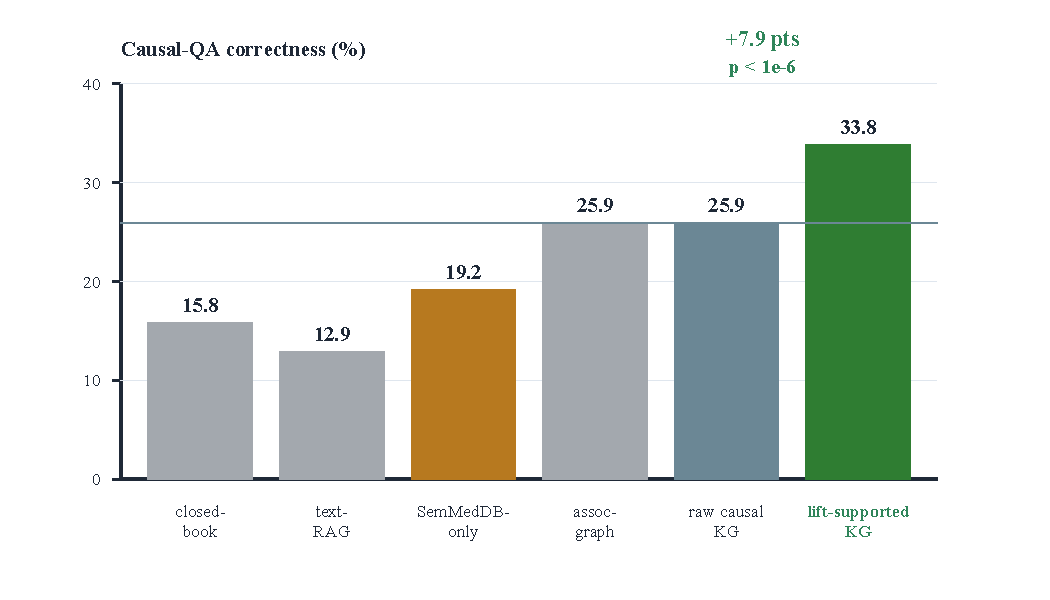
\includegraphics[width=0.92\textwidth]{fig_qa.pdf}
\caption{Causal-QA performance on held-out patients. Left: answer correctness. Right: unsupported hallucinated answers for systems where hallucination can be measured. The final system uses lift-only retrieval and demotes candidates that fail the causal screen. The main downstream effect is fewer unsupported hallucinated answers at fixed recall; the exact-accuracy change over lift-only is a small non-significant trend.}
\label{fig:qa}
\end{figure}

\subsection{Analysis of the gain} 
This experiment evaluates the retrieval utility of EHR support filtering rather than causal truth. The questions are forward-directed, so their direction is fixed by the query template. Improvements should therefore come from presenting better supported candidate causes or effects to the generator, not from proving that the retrieved relation is causally true. Lift-only retrieval is the appropriate base after the audit because it keeps the extractor's text-derived direction and avoids the unsupported coding-order temporal orientation. Causal demotion then makes a conservative ordering change: candidates that pass or cannot be tested by the causal screen remain ahead of candidates that fail it, while the same top-12 candidate set is preserved. The observed effect is therefore best interpreted as improved evidence discipline: faithfulness improves and unsupported hallucination decreases, while exact-concept accuracy shows only a small non-significant trend.
%This experiment probes the EHR-support filtering part of the audit. The questions are forward, so direction is fixed, and useful gains should come from showing the generator better supported candidate causes rather than from proving causal truth. Lift-only retrieval is the honest base because it keeps the extractor's direction and does not use the refuted coding-order temporal signal. Causal demotion then makes one conservative change: candidates that look supported by raw lift but fail the causal screen are moved to the bottom of the same top-12 list. This keeps recall fixed but reduces the chance that the generator follows a confounded or weakly supported candidate. The resulting gain is therefore best interpreted as better evidence discipline. It mainly improves faithfulness and hallucination, with a smaller non-significant trend in exact concept accuracy.


%\smallskip\noindent\textbf{Support filtering does not trade away recall.} Filtering candidates by lift could remove reference answers. In this benchmark it does not: the reference answer is present in the retrieved candidate set for 86.3\% of items under lift-only retrieval, versus 72.3\% for the raw-causal graph, 72.7\% for the associative graph, and 23.9\% for SemMedDB-only retrieval. Demotion preserves the same 86.3\% recall because it changes the order of the retrieved evidence rather than the candidate set. The generator therefore still sees the supported answer, but it is less distracted by candidates that fail the causal screen.
\smallskip\noindent\textbf{Recall is preserved.}
A potential risk of support filtering is that it may remove reference answers. In this benchmark, lift-only retrieval instead increases candidate recall: the reference answer appears in the retrieved candidate set for 86.3\% of items, compared with 72.3\% for raw-causal retrieval, 72.7\% for the associative graph, and 23.9\% for SemMedDB-only retrieval. Demotion preserves the same 86.3\% recall because it reorders the retrieved evidence without changing the candidate set. Thus, the generator still sees the supported answer but is less exposed to candidates that fail the causal screen.

%\smallskip\noindent\textbf{By question type.} WHATCAUSES is harder than WHY for every system (26.0\% vs.\ 48.5\% for ours). This follows from its one-to-many nature: a cause has many clinically valid effects, so matching a single reference effect undercounts all systems. The demotion variant improves both question types over the lift-only base.
\smallskip\noindent\textbf{Question-type effects.} WHATCAUSES is harder than WHY for every system. For our final system, accuracy is 26.0\% for WHATCAUSES and 48.5\% for WHY. This is expected because WHATCAUSES is more one-to-many: a single cause may lead to multiple clinically plausible effects, while the benchmark accepts only one reference concept. The demotion variant nevertheless improves both question types over the lift-only base.


\smallskip\noindent\textbf{Error analysis.} Three modes account for most residual errors. First, the system may name a clinically valid sibling of the reference concept and be marked wrong by exact-concept matching. This is the largest class. Second, retrieval gaps remain: for $\sim$22\% of items no graph surfaces the reference cause among its top candidates, capping achievable accuracy. Third, text-RAG and, to a lesser degree, the raw-causal graph sometimes answer a salient but wrong concept drawn from a noisy evidence list. This explains why text-RAG falls below the no-retrieval baseline. As a sanity check, stricter text-only variants in the same harness did not close the gap: a top-40 TF-IDF retriever restricted to causal-cue sentences reached 13.9\% overall, and a MiniLM sentence-retrieval variant reached 13.1\%, both below closed-book.

\section{Discussion and Limitations}
\noindent\textbf{Practical recommendations.} The audit yields four practical rules. First, use within-admission co-occurrence lift as an EHR support filter before retrieval. Second, do not orient candidates by diagnosis-coding order. Third, if a richer causal screen is available, use it to demote failed candidates rather than to replace the retrieval list. Fourth, treat literature corroboration (e.g.\ SemMedDB) as a confidence tier with limited coverage.

\noindent\textbf{On the temporal hazard.} Coding timestamps often reflect documentation rather than onset, a known problem in structured causal discovery~\cite{shen2021causaldiscovery}. We quantify this hazard for text-mined candidates: the naive coding-order signal agrees with neither the extractor nor the literature reference. This does not reject all temporal methods. It only shows that uncorrected cross-admission coding order is a weak independent direction signal.

\noindent\textbf{Threats to validity.} The QA reference is EHR-supported by construction and therefore overlaps the lift-supported graph. Because the raw-causal baseline contains a \emph{superset} of those candidates, the comparison still tests the effect of removing unsupported neighbours. It remains a coupled benchmark-method evaluation, not independent causal validation of lift. Population-level lift uses all patients' structured codes; a train-only estimate would be stricter. We also do not yet report a lift-threshold sensitivity sweep or a full evaluation of stronger clinical text retrieval baselines, including BM25, domain-specific dense retrieval, and hybrid retrieval. The lift-only condition includes lift scores, so the ablation tests the deployed support-aware retrieval recipe. Causal demotion should be read as evidence ordering, not causal proof. Its clearest effect is improved faithfulness and reduced hallucination; exact accuracy trends upward but is not significant.

\noindent\textbf{Other limitations.} We use one 7B open model and English ICU notes. MIMIC-III tests whether the audit signals replicate across an older EHR release; it is not a second full QA benchmark. Absolute QA numbers are modest, and the main downstream effect is reduced unsupported hallucination. The text-RAG row is not intended to represent the strongest possible clinical text retriever. We include two stricter text-only sanity checks in the same harness, but we do not claim to exhaust strong clinical text retrieval baselines such as BM25, domain-specific dense retrieval, or hybrid retrieval. The direct comparison with raw-causal retrieval is therefore the cleaner ablation for our main claim. Lift covers diagnosis-coded endpoints; prescriptions, adverse events, clinical findings, and multi-hop chains require richer validators. SemMedDB covers only a minority of candidates. Co-occurrence lift is an association signal: it supports an extracted candidate but cannot establish a true causal relation.

\noindent\textbf{Released artifacts.} The \href{https://anonymous.4open.science/r/clinical-causal-kg-artifact-C950/}{anonymous artifact package} provides the code, paper source, figures, aggregate summaries, and MIMIC-III replication summary. Restricted MIMIC, UMLS, and SemMedDB materials are not redistributed. With credentialed access, the scripts regenerate the support-filtered KG, benchmark instances, and audit labels.

\section{Conclusion}
Text-mined clinical causal candidate KGs require auditing at two levels: patient-level support for extracted candidates and direction. Auditing three EHR and literature signals against independent literature evidence, we find that co-occurrence lift provides useful EHR support but does not prove causal truth, whereas cross-admission coding order is unreliable as an independent EHR direction signal. Literature corroboration helps with direction but covers only a minority of candidates. The MIMIC-III replication recovers the same qualitative pattern, suggesting that the conclusion is not an artifact of a single MIMIC release. Text-mined clinical causal candidate KGs are therefore best treated as EHR-supported but direction-uncertain. In a controlled causal-RAG ablation, lift-only retrieval is the appropriate base after the temporal audit, and conservative causal demotion reduces unsupported hallucinated answers from 17.3\% to 6.1\% while preserving recall. More broadly, the results show why support signals should be audited against an independent reference before they are used to support, orient, or rank causal candidates. The same recipe can be applied to other note corpora and to richer validators, including onset-corrected timing, prescription signals, and multi-hop causal chains.

\begingroup
\let\oldthebibliography\thebibliography
\let\endoldthebibliography\endthebibliography
\renewenvironment{thebibliography}[1]{%
  \oldthebibliography{#1}%
  \footnotesize
  \setlength{\itemsep}{0pt}%
  \setlength{\parsep}{0pt}%
}{\endoldthebibliography}
\bibliographystyle{splncs04}
\bibliography{references}
\endgroup
\end{document}
